\begin{document}

% Lecture Notes: Genome Assembly

\section{Introduction to Genome Assembly}
Genome assembly and read mapping represent two fundamental approaches in bioinformatics for analyzing sequencing data. While mapping relies on an existing reference, de novo assembly attempts to reconstruct the genome from scratch, making it computationally challenging but essential for species without a known reference genome. 

\begin{important}
    \textbf{De novo Genome Assembly}: The computational process of piecing together a complete genome sequence from a large collection of short, randomly generated DNA fragments ("reads") without the use of a reference genome.
\end{important}

\begin{important}
    \textbf{Read Mapping}: The process of aligning short sequencing reads to a known reference genome to identify their origin and detect variations (e.g., mutations or structural variants).
\end{important}

\subsection{Sequencing Strategies: Single-end vs. Paired-end}
When modern high-throughput platforms (Next-Generation Sequencing, NGS) generate reads, they sequence specific portions of DNA fragments. We can categorize the sequencing strategies into two main types:

\begin{itemize}
    \item \textbf{Single-end sequencing}: Only one end of the DNA fragment is sequenced for a specific number of bases (e.g., 100-200 bp). This approach is sufficient for simpler tasks like ChIP-seq (identifying transcription factor binding sites).
    \item \textbf{Paired-end sequencing}: Both ends of a single DNA fragment are sequenced in opposite directions. Because the fragments are size-selected during preparation (e.g., distributed around an average length of 800 bases), we know the approximate distance between the resulting two reads. 
\end{itemize}

\sta Paired-end sequencing provides critical structural context. If two paired reads map to a reference genome much further apart than their expected fragment length, it strongly indicates a structural variant, such as a deletion in the sequenced individual.

% [IMAGE: A diagram showing paired-end and single-end reads mapping to a reference genome, illustrating how paired reads span unknown intervening sequences and can highlight translocations or deletions if mapped unusually far apart.]

\section{Sequencing Data: Models and Intuition}
To understand the complexity of genome assembly, we rely on probabilistic models. The process of shotgun sequencing randomly samples bases across the genome millions of times.

\subsection{Modeling Coverage Depth}
Let us define the fundamental variables used to model sequencing data:
\begin{itemize}
    \item \( G \): Genome size (e.g., \( 3.2 \times 10^9 \) for the human genome).
    \item \( L \): Read length (e.g., 100 or 200 bases depending on the specific sequencing run).
    \item \( N \): Total number of sequenced reads.
    \item \( n_b \): Total number of sequenced bases, easily calculated as \( n_b = N \times L \).
    \item \( \lambda \): Average coverage (or mean sequencing depth), representing the expected number of times a single base in the genome is sequenced.
\end{itemize}

We can calculate the average coverage depth per base as:
\begin{equation}
    \lambda = \frac{n_b}{G} = \frac{N \times L}{G} \label{eq:coverage}
\end{equation}

\textbf{Example:}
How many reads are required to cover the human genome at an average depth of 10x (\( \lambda = 10 \)), assuming a read length (\( L \)) of 200 bases?
We rearrange equation \eqref{eq:coverage} to solve for \( N \):
\begin{align*}
    N &= \frac{\lambda \times G}{L} \\
    N &= \frac{10 \times (3 \times 10^9)}{200} = 150,000,000 \text{ reads}
\end{align*}
This calculation illustrates the massive scale of modern sequencing: achieving a 10x coverage requires 150 million reads, while a high-quality 30x coverage requires nearly half a billion reads.

\subsection{The Poisson Distribution for Base Coverage}
The sampling of DNA fragments is fundamentally a random process involving independent and identically distributed events. Therefore, the distribution of coverage depth across the genome is well-modeled by a Poisson distribution.

\begin{important}
    \textbf{Poisson Distribution for Base Coverage}: Expresses the probability \( P(X=k) \) that a specific genomic position is covered by exactly \( k \) reads, given a mean sequencing depth \( \lambda \):
    \[ P(X = k) = \frac{e^{-\lambda} \lambda^k}{k!} \]
\end{important}

Using this model, we can estimate the probability that a given base is \textit{never} sequenced (\( k=0 \)):
\[ P(X = 0) = \frac{e^{-\lambda} \lambda^0}{0!} = e^{-\lambda} \]
Consequently, the probability of a base being covered at least once is:
\[ P(X > 0) = 1 - e^{-\lambda} \]

\sta This model highlights a critical limitation of sequencing: covering 100\% of the genome requires an infinite coverage depth, as \( e^{-\lambda} \) only approaches zero asymptotically. In practice, gaps are unavoidable.

To estimate the minimum average depth required to cover 99\% of the genome at least once (\( P(X > 0) = 0.99 \)):
\begin{align*}
    1 - e^{-\lambda} &= 0.99 \\
    e^{-\lambda} &= 0.01 \\
    -\lambda &= \ln(0.01) \approx -4.605
\end{align*}
This result mathematically explains the historical goal of achieving approximately 6x coverage in initial Sanger sequencing projects.

\subsection{k-mers and Genome Size Estimation}
While average base coverage (\( \lambda \)) requires knowing the genome size \( G \), we can estimate \( G \) directly from raw read data using k-mers. 

\begin{important}
    \textbf{k-mer}: A continuous subsequence of length \( k \) extracted from a longer sequence (e.g., a read). 
\end{important}

For a single read of length \( L \), the number of possible k-mers is \( L - k + 1 \).
For a dataset of \( N \) reads, the total number of k-mers is:
\[ n_k = N \times (L - k + 1) \]

We can define k-mer coverage depth (\( d_k \)) as the average number of times a unique k-mer appears in the dataset. The relationship between base coverage (\( \lambda \)) and k-mer coverage (\( d_k \)) is strictly a geometric ratio:
\[ \frac{\lambda}{d_k} = \frac{n_b / G}{n_k / G} = \frac{L}{L - k + 1} \]

If \( k \) is sufficiently large (e.g., \( k=50 \)), most k-mers will be unique across the genome. By counting the frequencies of all k-mers in the dataset and finding the peak of this empirical distribution, we can identify \( d_k \). We can then estimate the unknown genome size \( G \) as:
\[ G \approx \frac{n_k}{d_k} \]
This technique is exceptionally powerful for characterizing novel species before assembly begins.

% [IMAGE: A plot showing the distribution of k-mer frequencies. The x-axis represents the depth of coverage (number of times a k-mer is observed), and the y-axis represents the number of distinct k-mers. A clear peak is visible, representing the mean k-mer coverage depth, d_k. A smaller peak near zero represents unique sequencing errors.]

\section{Genome Assembly and Contigs}
Because achieving 100\% base coverage is statistically impossible, genome assembly does not yield a single unbroken sequence. Instead, it yields a collection of contiguous sequences separated by gaps.

\begin{important}
    \textbf{Contig}: A contiguous sequence formed by piecing together overlapping sequencing reads. Contigs represent the best possible reconstruction of the original DNA sequence, though their absolute order and orientation remain unknown without further scaffolding.
\end{important}

\subsection{Expected Number and Size of Contigs}
We can calculate the expected number of contigs by counting the "rightmost reads" in an assembly. A read is the rightmost read of a contig if no other read starts within its interval of length \( L \).

The expected number of reads starting at any given base is \( N / G \).
In an interval of length \( L \), the expected number of read starts is:
\[ L \times \frac{N}{G} = \lambda \]
The probability that \textit{zero} reads start in this interval is again given by the Poisson distribution: \( e^{-\lambda} \).

Because there are \( N \) total reads, the expected number of rightmost reads (and thus, the expected number of contigs) is:
\[ \text{Expected Contigs} = N e^{-\lambda} \]
The expected number of reads per contig is \( \frac{N}{N e^{-\lambda}} = e^\lambda \).

The expected total fraction of the genome covered by contigs is \( (1 - e^{-\lambda}) \cdot G \). Therefore, the expected size of a single contig is:
\[ \text{Expected Contig Size} = \frac{(1 - e^{-\lambda}) \cdot G}{N e^{-\lambda}} \]

\textbf{Example:}
Given a human genome (\( G = 3 \times 10^9 \)), reads of length \( L = 500 \), and a target coverage \( \lambda = 6 \).
\begin{enumerate}
    \item Reads required: \( N = \frac{6 \times 3 \times 10^9}{500} = 36 \text{ million reads} \).
    \item Expected contigs: \( 36,000,000 \times e^{-6} \approx 89,235 \text{ contigs} \).
    \item Average contig length: \( \approx 33,536 \text{ bases} \).
\end{enumerate}
This demonstrates that even with robust coverage, the genome remains heavily fragmented into thousands of pieces.

\subsection{Contigs and Read Overlaps}
The previous derivation assumed that an overlap of just 1 nucleotide was sufficient to join reads. In reality, a 1-bp overlap has a 25\% chance of occurring randomly. We require a substantial minimum overlap, defined as a fraction \( \theta \) of the read length \( L \). 

When we require an overlap of \( \theta L \) nucleotides, a read only represents the end of a contig if no other read starts within the leftmost \( (1 - \theta) L \) portion of its span. Adjusting the Poisson probability, the expected number of contigs becomes:
\[ \mathbb{E}[\# \text{ contigs}] = N e^{-(1 - \theta) \lambda} \]
As \( \lambda \) increases, the number of contigs drops (better assembly). As \( \theta \) increases (requiring stricter overlaps to avoid false joins), the assembly breaks into more, smaller contigs.

\begin{important}
    \textbf{N50 Metric}: A statistical measure of assembly quality. If all contigs are sorted from largest to smallest, the N50 is the length of the contig at which the cumulative length covers exactly 50\% of the total genome size. A higher N50 indicates a more contiguous, higher-quality assembly.
\end{important}

\section{Graph Theory in Genome Assembly}
Modern genome assembly relies heavily on Graph Theory, tracing its conceptual roots back to Leonhard Euler's 1736 analysis of the Königsberg Bridge Problem. The computational objective is to take a massive collection of short NGS reads and find a path through overlapping elements that represents the original genome sequence.

\subsection{The Naive Approach: Hamiltonian Path}
If we break our reads into a collection of unique k-mers, we could naively assign each k-mer to a \textbf{node} in a graph. We place \textbf{directed edges} between nodes where the suffix of the first k-mer perfectly matches the prefix of the second k-mer.

To reconstruct the genome under this model, we must visit every k-mer exactly once.
\begin{important}
    \textbf{Hamiltonian Path}: A path in a directed or undirected graph that visits every vertex (node) exactly once. (It is not required to traverse all edges).
\end{important}

\sta \textbf{Critical Limitation:} Finding a Hamiltonian Path is an \textbf{NP-complete} problem. In the context of millions of reads, checking solutions scales exponentially ($O(2^N)$ depending on formulation), making it entirely computationally infeasible for whole-genome assembly.

\subsection{The De Bruijn Graph (DBG) Approach: Eulerian Path}
To circumvent the computational limits of the Hamiltonian approach, modern assemblers redefine the graph structure.

In a \textbf{De Bruijn Graph (DBG)}:
\begin{itemize}
    \item \textbf{Edges} represent the k-mers (the observed sequences).
    \item \textbf{Nodes} represent the (k-1)-mer prefixes and suffixes of those k-mers.
\end{itemize}

Construction of a DBG proceeds as follows:
\begin{enumerate}
    \item Extract all k-mers from the read data.
    \item For each k-mer, create a directed edge originating from a node labeled with its $(k-1)$ prefix and pointing to a node labeled with its $(k-1)$ suffix.
    \item \textbf{Merge} all nodes sharing identical $(k-1)$ labels into a single node, while \textbf{retaining all connecting edges}.
\end{enumerate}

To reconstruct the genome from a DBG, we must utilize all of our observed k-mers, which means we must traverse every \textit{edge} exactly once.
\begin{important}
    \textbf{Eulerian Path}: A path in a graph that visits every edge exactly once. Nodes may be visited multiple times. If the path ends at the starting node, it is an Eulerian Cycle.
\end{important}

\sta \textbf{Advantage:} Unlike the Hamiltonian path problem, finding an Eulerian path is solvable in \textbf{linear time} ($\mathcal{O}(E)$) using algorithms like Hierholzer's. This is the cornerstone of modern Next-Generation Sequence assembly.

\subsection{Graph Compression}
After a basic DBG is built, it often contains long chains of unambiguous paths—sequences of nodes where each node has an in-degree of 1 and an out-degree of 1. Because there are no diverging branches, these paths can be \textbf{compressed}.
Nodes along an unambiguous path are merged, and their labels concatenated, forming longer contiguous sequences. This drastically reduces the graph size without altering the topological routing options.

% [IMAGE: A sequence of De Bruijn graph diagrams transitioning from isolated edges representing overlapping word-fragments (like 'the more things', 'more things you'), to merged nodes sharing common prefixes/suffixes, and finally to a compressed path merging nodes into longer continuous phrases.]

\section{Finding Eulerian Paths: Hierholzer's Algorithm}
Before searching for an Eulerian path, we must confirm the graph is traversable. The traversability is determined purely by the \textbf{degree} of its vertices.

\textbf{Property (Eulerian Traversability in Directed Graphs):}
\begin{itemize}
    \item \textbf{Eulerian Cycle}: Exists if and only if every vertex has identical in-degree and out-degree ($In = Out$).
    \item \textbf{Eulerian Path}: Exists if and only if exactly one vertex has $(Out - In = 1)$ (the starting node) and exactly one vertex has $(In - Out = 1)$ (the ending node), while all other vertices have $In = Out$.
\end{itemize}

\subsection{Algorithm Execution}
Hierholzer's Algorithm extracts an Eulerian path in $O(E)$ time. It relies on a stack data structure (Last In, First Out) to trace paths and backtrack when dead-ends are reached.

\begin{enumerate}
    \item \textbf{Initialize} two stacks: \texttt{tpath} (temporary path) and \texttt{epath} (final Eulerian path solution).
    \item \textbf{Identify Starting Node}: Choose vertex $v$ with $Out - In = 1$ (or any node if searching for a cycle) and push $v$ to \texttt{tpath}.
    \item \textbf{Examine Top Node}: Let $u$ be the node at the top of \texttt{tpath}.
    \item \textbf{Check Outgoing Edges}:
        \begin{itemize}
            \item If $u$ has unvisited outgoing edges: Randomly select an outgoing edge to node $x$. Push $x$ to \texttt{tpath} and delete/mark the edge $(u,x)$ as visited.
            \item If $u$ has \textbf{no} unvisited outgoing edges: Pop $u$ off \texttt{tpath} and push it onto \texttt{epath}.
        \end{itemize}
    \item \textbf{Repeat} Step 3 until \texttt{tpath} is completely empty.
    \item The final Eulerian path resides in \texttt{epath}, reading from top to bottom.
\end{enumerate}

\textbf{Example:} Walkthrough of Hierholzer's logic on a small graph.
\textit{Illustration of Stack Backtracking Mechanism}:
\begin{enumerate}
    \item We start tracing a path and pushing nodes to \texttt{tpath}.
    \item Eventually, we hit the \textbf{end node}. By definition, the end node is the first node we encounter from which we have exhausted all outgoing paths (because its In-degree > Out-degree). 
    \item We pop this end node from \texttt{tpath} and push it to \texttt{epath} (it becomes the bottom of the final stack).
    \item The algorithm now backtracks by checking the new top of \texttt{tpath}. If there are unused branch paths, it explores them. If those sub-paths hit dead ends, they are recursively pushed to \texttt{epath}.
    \item The very last node popped from \texttt{tpath} to \texttt{epath} will be the starting node, guaranteeing a complete traversal.
\end{enumerate}

% [IMAGE: A stack-based diagram showing tpath and epath at various stages. Nodes are added to tpath until a dead end (node 6) is reached. Node 6 is moved to epath, and the algorithm backtracks to node 4, exploring alternative branches before recursively moving elements to epath until tpath is empty.]

\section{Practical Problems in Genome Assembly}
While the Eulerian path on a De Bruijn graph elegantly handles idealized sequencing, real biological data introduces several complicating factors.

\subsection{Selecting K-mer Size ($k$) and Memory Constraints}
The size of $k$ dictates the overlap required to merge reads (a $k$-mer implies a $k-1$ overlap).
\begin{itemize}
    \item \textbf{If $k$ is too small}: Almost no k-mers are unique. The graph becomes hyper-connected with false overlaps, leading to massive ambiguity and fragmented contigs.
    \item \textbf{If $k$ is too large}: Overlap requirements become too stringent. Because sequencing reads have random starting positions, finding reads with identical, massive k-mers requires prohibitively high sequencing depth. Without it, the graph breaks into unconnected islands.
\end{itemize}
\sta Furthermore, memory usage scales as $\mathcal{O}(n \cdot k)$. Storing billions of nodes requires substantial RAM. Computational implementations often compress nucleotides into 2-bit notation (\texttt{A=00, C=01, G=10, T=11}) to pack 4 bases per byte and constrain memory overhead.

\subsection{Sequencing Errors}
A single base error in a read of length $L$ corrupts exactly $k$ different k-mers (since the erroneous base shifts through $k$ positions).
\begin{itemize}
    \item These corrupted k-mers will typically appear only once in the dataset (frequency = 1), whereas genuine k-mers appear with a frequency roughly equal to the average coverage depth $\lambda$.
    \item This creates isolated "spurs" or "bubbles" in the DBG. A common heuristic is to simply prune nodes/edges from the graph that have a frequency count beneath a specific threshold.
\end{itemize}

\subsection{Repetitive Regions and Strand Ambiguity}
Repeats (e.g., tandem repeats like \texttt{CATCATCAT...}) collapse into a single highly traversed loop in the DBG. If the repeat is longer than the chosen $k$-mer size, the DBG cannot resolve where the read entered or exited the repeat, destroying contiguity.

Finally, DNA is double-stranded. A shotgun sequencing protocol typically selects fragments randomly from both the forward and reverse strands. Assemblers must treat every k-mer and its reverse-complement as equivalent nodes to ensure both strands map to the same genomic assembly path. 

\subsection{Diploidy and Heterozygosity}
Most complex organisms, including humans, possess diploid genomes, meaning they have two homologous copies of every chromosome. While these copies are largely identical, they contain naturally occurring variations, such as Single Nucleotide Polymorphisms (SNPs). 

If a specific genomic position has an \texttt{A} on the maternal chromosome and a \texttt{G} on the paternal chromosome, the sequencing reads will capture both alleles. Assuming an average coverage of 30x, we would expect roughly 15 reads supporting the \texttt{A} allele and 15 reads supporting the \texttt{G} allele.

In the De Bruijn Graph, this variation manifests as a structural \textbf{bubble}:
\begin{itemize}
    \item The graph path splits into two parallel branches at the variant position.
    \item One branch contains the k-mers featuring the \texttt{A} allele; the other contains the k-mers featuring the \texttt{G} allele.
    \item After the $k$ positions spanned by the variant, the two paths merge back into a single node representing the identical downstream sequence.
\end{itemize}
\sta Assemblers must be designed to recognize and resolve these "bubbles" so they do not artificially duplicate genomic regions or break contiguity.

\section{Assembly Strategies: Overlap-Layout-Consensus vs. De Bruijn Graphs}
Historically, genome assembly algorithms evolved to match the predominant sequencing technologies of their time. The transition from long-read (Sanger) to short-read (Next-Generation Sequencing) technologies necessitated a paradigm shift in algorithm design.

\subsection{Overlap-Layout-Consensus (OLC)}
The Overlap-Layout-Consensus (OLC) approach was the gold standard during the Human Genome Project, which relied on Sanger sequencing reads that were hundreds or thousands of bases long.

\begin{important}
    \textbf{Overlap-Layout-Consensus (OLC)}: An assembly method that directly compares all reads against all other reads to identify overlaps, constructs a layout of how the reads tile together, and derives a final consensus sequence.
\end{important}

The OLC pipeline proceeds in three steps:
\begin{enumerate}
    \item \textbf{Overlap}: Compute all-against-all pairwise alignments to find overlaps between reads.
    \item \textbf{Layout}: Form a graph where reads are nodes and overlaps are edges, then untangle this graph to find an ordered layout of reads.
    \item \textbf{Consensus}: Derive the most likely true sequence by taking the majority vote of the aligned bases in the layout.
\end{enumerate}

\sta \textbf{Computational Bottleneck:} The overlap phase requires $\mathcal{O}(N^2)$ pairwise comparisons, where $N$ is the number of reads. While feasible for the thousands of long reads in Sanger sequencing, applying OLC to the hundreds of millions of short reads generated by NGS is computationally explosive.

\subsection{Case Study: The Greedy Overlap Failure (The Dr. Seuss-Ome)}
To intuitively understand why OLC/Greedy overlap approaches fail on repetitive short-read data, and why De Bruijn Graphs succeed, we analyze a text-based analogy using a quote from Dr. Seuss.

\textbf{Example:} Reconstructing the "Dr. Seuss-Ome"
Let our target genome be the following sentence, and our reads be 3-word fragments ($k=3$):
\textit{"The more that you read, the more things you will know. The more that you learn, the more places you'll go."}

Imagine the text is shredded into all possible 3-word combinations. We attempt to reconstruct the text using a \textbf{Greedy Reconstruction} strategy (a naive OLC approach):
\begin{enumerate}
    \item We randomly select a starting fragment: \texttt{"more things you"}.
    \item We search for a fragment whose first 2 words match our last 2 words. We find \texttt{"things you will"} and append it.
    \item We continue greedily: \texttt{"you will know"} $\rightarrow$ \texttt{"will know The"} $\rightarrow$ \texttt{"know The more"}.
    \item We arrive at the 2-word suffix \texttt{"the more"}. 
\end{enumerate}

At \texttt{"the more"}, the greedy algorithm faces a critical ambiguity. There are four valid fragments in our dataset that start with \texttt{"the more"}:
\begin{itemize}
    \item \texttt{"the more that"} (occurs twice)
    \item \texttt{"the more things"}
    \item \texttt{"the more places"}
\end{itemize}
Because a greedy algorithm makes immediate, finalized choices based on local overlap, picking the wrong branch at this juncture will inevitably lead to a \textit{chimeric} (misassembled) sequence that does not reflect the original text. The algorithm gets stuck or generates an incorrect genome.

\subsection{De Bruijn Graph (DBG) Resolution}
Instead of attempting to immediately sequence the fragments, the De Bruijn Graph maps out the entire topological structure of the data before committing to a path.

Applying the DBG rules to the Dr. Seuss-Ome:
\begin{itemize}
    \item \textbf{Edges}: 3-word fragments (e.g., \texttt{the $\rightarrow$ more $\rightarrow$ that}).
    \item \textbf{Nodes}: 2-word prefixes and suffixes.
\end{itemize}

When constructing the graph, the phrase \texttt{"the more"} becomes a single, highly-traversed node. Instead of forcing a premature guess, the DBG explicitly models the ambiguity by assigning this node an out-degree of 4:

\begin{center}
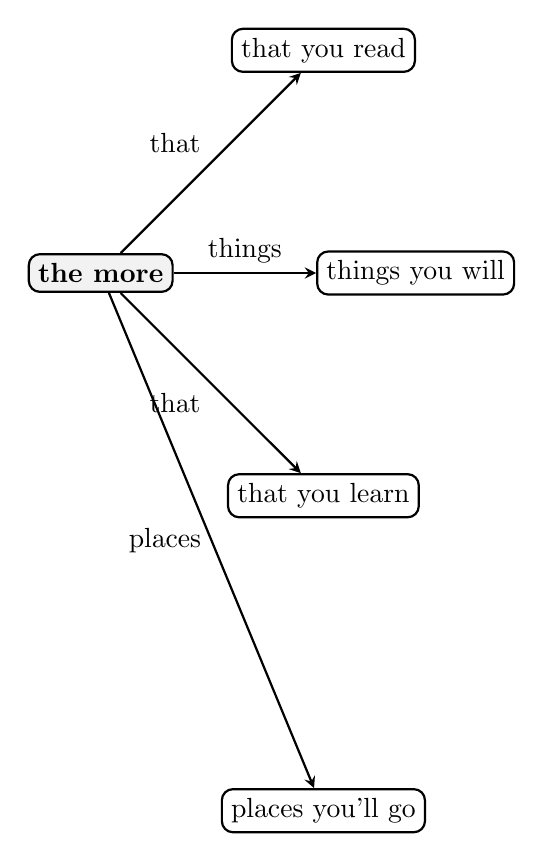
\begin{tikzpicture}[->, >=stealth, node distance=4cm, thick]
    \node[draw, rectangle, rounded corners, fill=gray!10] (the_more) {\textbf{the more}};
    \node[draw, rectangle, rounded corners] (that_read) [above right of=the_more] {that you read};
    \node[draw, rectangle, rounded corners] (things_know) [right of=the_more] {things you will};
    \node[draw, rectangle, rounded corners] (that_learn) [below right of=the_more] {that you learn};
    \node[draw, rectangle, rounded corners] (places_go) [below of=that_learn] {places you'll go};

    \path
    (the_more) edge node[above left] {that} (that_read)
    (the_more) edge node[above] {things} (things_know)
    (the_more) edge node[below left] {that} (that_learn)
    (the_more) edge node[left] {places} (places_go);
\end{tikzpicture}
\end{center}
% [IMAGE: A diagram showing a central node labeled "the more" branching outwards into four distinct paths representing the different continuations of the sentence, explicitly capturing the structural ambiguity rather than forcing a greedy choice.]

\textbf{Graph Compression on the DBG:}
Once the global structure is built, the DBG reveals long sequences of unambiguous paths. For instance, once a path enters \texttt{"things"}, it must traverse \texttt{"you"} $\rightarrow$ \texttt{"will"} $\rightarrow$ \texttt{"know."}. 
The compression algorithm merges these nodes (which have in-degree 1 and out-degree 1) into a single, extended node: \texttt{"things you will know."}. 

By mapping the entire problem space and compressing unambiguous paths, the Eulerian path algorithm (like Hierholzer's) can traverse the graph, evaluating global connections to reconstruct the original text with vastly higher accuracy than a greedy layout approach.

\section{From Contigs to Scaffolds}
The final output of the Hierholzer traversal over a De Bruijn Graph is a set of \textbf{contigs}. However, as previously derived, even high-coverage assemblies contain gaps due to random sampling, sequencing errors, or unresolved repeats. We are left with thousands of disconnected contigs whose relative order and orientation are unknown.

To bridge these gaps, we utilize the structural information provided by \textbf{paired-end sequencing}.

\begin{important}
    \textbf{Scaffold}: A higher-order assembly structure consisting of ordered and oriented contigs separated by gaps of known (or estimated) length.
\end{important}

If one read of a paired-end fragment maps to the tail of Contig A, and its paired read maps to the head of Contig B, we establish a definitive link. Because we know the approximate total length of the original DNA fragment (e.g., $800 \text{ bp}$), and the lengths of the mapping reads (e.g., $200 \text{ bp}$ each), we can estimate the distance of the unknown gap separating Contig A and Contig B. 

\sta While De novo assembly rarely produces a single, complete chromosome, scaffolding drastically reduces fragmentation, bridging isolated contigs into large, structurally accurate genomic frameworks.

\end{document}